\documentclass[aspectratio=169,10pt]{beamer}

% Theme & Styling
\usetheme{Madrid}
\usecolortheme{whale}

% Standard Packages (Overleaf Compatible)
\usepackage[utf8]{inputenc}
\usepackage[T1]{fontenc}
\usepackage{amsmath,amssymb,amsfonts}
\usepackage{booktabs}
\usepackage{colortbl}
\usepackage{tikz}
\usetikzlibrary{shapes,arrows.meta,positioning,shadows,calc}
\usepackage{hyperref}
\usepackage{microtype}
\usepackage{xcolor}

% Custom Color Palette (IBM / Deep Police Intelligence Theme)
\definecolor{NavyBlue}{RGB}{15, 34, 64}
\definecolor{CrimsonAlert}{RGB}{195, 33, 72}
\definecolor{AlertAmber}{RGB}{220, 130, 20}
\definecolor{SuccessGreen}{RGB}{24, 134, 75}
\definecolor{SlateGray}{RGB}{100, 110, 125}
\definecolor{LightBg}{RGB}{245, 247, 250}
\definecolor{CardBg}{RGB}{238, 242, 248}

\setbeamercolor{palette primary}{bg=NavyBlue,fg=white}
\setbeamercolor{palette secondary}{bg=NavyBlue!85,fg=white}
\setbeamercolor{palette tertiary}{bg=NavyBlue!70,fg=white}
\setbeamercolor{structure}{fg=NavyBlue}
\setbeamercolor{frametitle}{bg=NavyBlue,fg=white}
\setbeamercolor{block title}{bg=NavyBlue,fg=white}
\setbeamercolor{block body}{bg=CardBg,fg=black}
\setbeamercolor{block title alerted}{bg=CrimsonAlert,fg=white}
\setbeamercolor{block body alerted}{bg=CrimsonAlert!10,fg=black}
\setbeamercolor{block title example}{bg=SuccessGreen,fg=white}
\setbeamercolor{block body example}{bg=SuccessGreen!10,fg=black}

% Remove navigation symbols
\setbeamertemplate{navigation symbols}{}
\setbeamertemplate{headline}{}

% Custom Footline with Slide Counter
\setbeamertemplate{footline}{
  \leavevmode%
  \hbox{%
  \begin{beamercolorbox}[wd=.35\paperwidth,ht=2.5ex,dp=1ex,left,leftskip=1ex]{palette primary}%
    \textbf{Oculon} | Predictive Crime Intelligence
  \end{beamercolorbox}%
  \begin{beamercolorbox}[wd=.40\paperwidth,ht=2.5ex,dp=1ex,center]{palette primary}%
    Delhi Police ZIPNET $\rightarrow$ Proactive Patrol Allocation
  \end{beamercolorbox}%
  \begin{beamercolorbox}[wd=.25\paperwidth,ht=2.5ex,dp=1ex,right,rightskip=1ex]{palette primary}%
    \insertframenumber{} / \inserttotalframenumber
  \end{beamercolorbox}}%
  \vskip0pt%
}

% Title Metadata
\title[Oculon: Predictive Crime Hotspot Mapping Assistant]{\textbf{OCULON: Predictive Crime Hotspot Mapping Assistant}}
\subtitle{Transforming Delhi Police ZIPNET into Proactive Patrol Intelligence for the Station House Officer (SHO)}
\author[Team Oculon]{%
  \textbf{Abhyuday Mishra} (Team Lead - \texttt{abhymishrgkp@gmail.com})\\
  \vspace{0.15cm}
  {\footnotesize \textbf{Team Members:} Abhishek Kumar $\cdot$ Shivam Ahirwal $\cdot$ Aditya Soni}
}
\institute[DelhiHotspots\_ML]{%
  \textsf{IBM Bob AI Hackathon 2026} \\
  \textsf{Repository: \url{https://github.com/abhyudaymishr/oculon}}
}
\date{September 2026}

\begin{document}

% -----------------------------------------------------------------------------
% SLIDE 1: TITLE SLIDE
% -----------------------------------------------------------------------------
\begin{frame}[plain]
  \titlepage
\end{frame}

% -----------------------------------------------------------------------------
% SLIDE 2: THE PROBLEM STATEMENT & REAL-WORLD CONTEXT
% -----------------------------------------------------------------------------
\begin{frame}{The Real Case: Delhi ZIPNET vs. Proactive Policing}
  \begin{columns}[T]
    \begin{column}{0.48\textwidth}
      \begin{block}{\textbf{The ZIPNET Reality in Delhi NCR}}
        \begin{itemize}\itemsep=0.4em
          \item \textbf{Decades of Incident Sinks:} Over 142,000+ geo-tagged incident records (Missing Persons, Bodies, Vehicles, Mobiles).
          \item \textbf{No Predictive Intelligence:} Data remains purely archival; queried retrospectively after incidents occur.
          \item \textbf{Static Beat Patrols:} Constables and PCR vans walk fixed, legacy routes oblivious to emerging temporal concentrations.
        \end{itemize}
      \end{block}
    \end{column}

    \begin{column}{0.48\textwidth}
      \begin{alertblock}{\textbf{The Proven Benchmark: Bengaluru 2023}}
        \begin{itemize}\itemsep=0.4em
          \item \textbf{18\% Property Crime Reduction:} Demonstrated in test zones through algorithmic micro-patrol dynamic shifts.
          \item \textbf{The Core Need:} A lightweight assistant that takes 6 months of rolling station data and equips the \textbf{Station House Officer (SHO)} with automated weekly action briefs.
        \end{itemize}
      \end{alertblock}
    \end{column}
  \end{columns}

  \vspace{0.4cm}
  \begin{center}
    \colorbox{CardBg}{\parbox{0.95\textwidth}{\centering \textbf{Mission:} Build a Bob-powered Crime Intelligence Assistant that ingests 6-month historical incident streams, identifies spatiotemporal concentration patterns, predicts the \textbf{Top 5 at-risk micro-zones}, and auto-generates actionable patrol redeployment briefs for the SHO.}}
  \end{center}
\end{frame}

% -----------------------------------------------------------------------------
% SLIDE 3: SYSTEM ARCHITECTURE & BOB INTEGRATION
% -----------------------------------------------------------------------------
\begin{frame}{System Architecture: Bob-Powered Assistant \& MCP}
  \begin{center}
    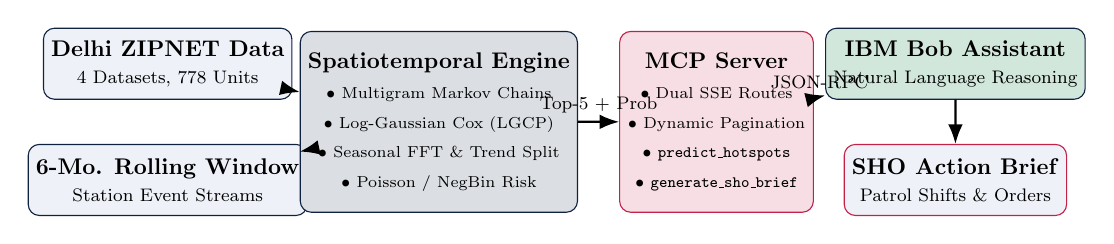
\begin{tikzpicture}[scale=0.82, every node/.style={transform shape, align=center}]
      % Ingestion Layer
      \node[draw=NavyBlue, fill=CardBg, rounded corners, minimum width=2.8cm, minimum height=1.1cm] (zipnet) at (0, 3) {\textbf{Delhi ZIPNET Data}\\\footnotesize 4 Datasets, 778 Units};
      \node[draw=NavyBlue, fill=CardBg, rounded corners, minimum width=2.8cm, minimum height=1.1cm] (stream) at (0, 1.2) {\textbf{6-Mo. Rolling Window}\\\footnotesize Station Event Streams};
      % Engine
      \node[draw=NavyBlue, fill=NavyBlue!15, rounded corners, minimum width=3.4cm, minimum height=2.8cm] (engine) at (4.2, 2.1) {%
        \textbf{Spatiotemporal Engine}\\[0.15em]
        \scriptsize $\bullet$ Multigram Markov Chains\\[0.1em]
        \scriptsize $\bullet$ Log-Gaussian Cox (LGCP)\\[0.1em]
        \scriptsize $\bullet$ Seasonal FFT \& Trend Split\\[0.1em]
        \scriptsize $\bullet$ Poisson / NegBin Risk%
      };
      % Protocol Layer
      \node[draw=CrimsonAlert, fill=CrimsonAlert!15, rounded corners, minimum width=3.0cm, minimum height=2.8cm] (mcp) at (8.5, 2.1) {%
        \textbf{MCP Server}\\[0.15em]
        \scriptsize $\bullet$ Dual SSE Routes\\[0.1em]
        \scriptsize $\bullet$ Dynamic Pagination\\[0.1em]
        \scriptsize $\bullet$ \texttt{predict\_hotspots}\\[0.1em]
        \scriptsize $\bullet$ \texttt{generate\_sho\_brief}%
      };
      % Bob Assistant & SHO Output
      \node[draw=NavyBlue, fill=SuccessGreen!20, rounded corners, minimum width=2.8cm, minimum height=1.1cm] (bob) at (12.2, 3) {\textbf{IBM Bob Assistant}\\\footnotesize Natural Language Reasoning};
      \node[draw=CrimsonAlert, fill=CardBg, rounded corners, minimum width=2.8cm, minimum height=1.1cm] (sho) at (12.2, 1.2) {\textbf{SHO Action Brief}\\\footnotesize Patrol Shifts \& Orders};
      % Connections
      \draw[-{Latex[length=2.5mm]}, thick] (zipnet) -- (engine);
      \draw[-{Latex[length=2.5mm]}, thick] (stream) -- (engine);
      \draw[-{Latex[length=2.5mm]}, thick] (engine) -- node[above]{\footnotesize Top-5 + Prob} (mcp);
      \draw[-{Latex[length=2.5mm]}, thick] (mcp) -- node[above]{\footnotesize JSON-RPC} (bob);
      \draw[-{Latex[length=2.5mm]}, thick] (bob) -- (sho);
    \end{tikzpicture}
  \end{center}

  \begin{exampleblock}{\textbf{Load-Bearing Bob Integration via Model Context Protocol (MCP)}}
    \small Bob communicates directly with Oculon's backend over Server-Sent Events (SSE). Bob asks for predictions, extracts mathematical probabilities, correlates seasonal festival calendars, and formats military-grade tactical patrol rosters.
  \end{exampleblock}
\end{frame}

% -----------------------------------------------------------------------------
% SLIDE 4: THE DATA FOUNDATION (778 ADMINISTRATIVE UNITS)
% -----------------------------------------------------------------------------
\begin{frame}{Data Foundation: Delhi NCR Multi-Domain Intelligence}
  \begin{table}
    \centering
    \small
    \begin{tabular}{lcccc}
      \toprule
      \textbf{Crime / Incident Category} & \textbf{Historical Depth} & \textbf{Total Records} & \textbf{Spatial Resolution} & \textbf{Model Entity Units} \\
      \midrule
      \rowcolor{CardBg} \textbf{Missing Persons (ZIPNET)} & 136 Months & 104,235 events & Police Station Polygons & 210 PS Jurisdictions \\
      \textbf{Unidentified Dead Bodies} & 53 Months & 9,892 events & Police Station Boundaries & 210 PS Jurisdictions \\
      \rowcolor{CardBg} \textbf{Vehicle Thefts (ZIPNET)} & 83 Months & 26,352 events & Metro Stations \& PINs & 259 Metros + 98 PINs \\
      \textbf{Stolen / Missing Mobiles} & 9 Months & 1,602 events & District Aggregates & City-Wide Temporal Rates \\
      \bottomrule
    \end{tabular}
  \end{table}

  \begin{columns}[T]
    \begin{column}{0.48\textwidth}
      \begin{block}{\textbf{Spatial Alignment \& Geocoding}}
        \footnotesize
        \begin{itemize}\itemsep=0.2em
          \item 778 canonical micro-units mapped via official Delhi GeoJSON shapefiles.
          \item Coordinate bounding box: Lat [$28.40^\circ, 28.88^\circ$ N], Lon [$76.84^\circ, 77.35^\circ$ E].
          \item Eliminates boundaries mismatch between transit corridors and jurisdiction lines.
        \end{itemize}
      \end{block}
    \end{column}

    \begin{column}{0.48\textwidth}
      \begin{block}{\textbf{6-Month Rolling Buffer Architecture}}
        \footnotesize
        \begin{itemize}\itemsep=0.2em
          \item Implements continuous rolling-origin retraining ($T-6 \to T-1$).
          \item Captures short-term displacement caused by previous police raids or metro line openings.
          \item Zero data leakage across forward evaluation horizons.
        \end{itemize}
      \end{block}
    \end{column}
  \end{columns}
\end{frame}

% -----------------------------------------------------------------------------
% SLIDE 5: MATHEMATICAL FORMULATION
% -----------------------------------------------------------------------------
\begin{frame}{Mathematical Engine: Multigram Markov + LGCP}
  \begin{columns}[T]
    \begin{column}{0.50\textwidth}
      \begin{block}{\textbf{1. Temporal Multigram Markov Transitions}}
        \footnotesize
        Arrival sequences $S_t$ conditioned on rolling $k$-order incident states ($k \in \{1, 2, 3\}$):
        \begin{equation*}
          P(S_t = s \mid S_{t-k:t-1}) = \frac{C(S_{t-k:t}) + \alpha}{\sum_{s'} [C(S_{t-k:t-1}, s') + \alpha]}
        \end{equation*}
        \textit{Captures multi-week persistence and rapid shifts in localized micro-zone repeat incidents.}
      \end{block}
    \end{column}

    \begin{column}{0.48\textwidth}
      \begin{block}{\textbf{2. Log-Gaussian Cox Process (LGCP)}}
        \footnotesize
        Continuous spatial intensity field $\Lambda(s)$ across coordinates $s \in \mathbb{R}^2$:
        \begin{equation*}
          \log \Lambda(s) = \mu(s) + \mathcal{G}(s)
        \end{equation*}
        where $\mathcal{G}(s) \sim \mathcal{GP}(0, K_\theta)$ with Mat\'ern / RBF kernel:
        \begin{equation*}
          K(s, s') = \sigma^2 \exp\left(-\frac{\|s - s'\|^2}{2\ell^2}\right)
        \end{equation*}
      \end{block}
    \end{column}
  \end{columns}

  \vspace{0.2cm}
  \begin{block}{\textbf{3. Overdispersed Negative Binomial Risk Probability}}
    \footnotesize
    Predicts probability of $y$ incidents in micro-zone $i$ with dispersion parameter $r$:
    \begin{equation*}
      P(Y_i = y \mid \mu_i, r) = \frac{\Gamma(y + r)}{y! \, \Gamma(r)} \left(\frac{r}{r + \mu_i}\right)^r \left(\frac{\mu_i}{r + \mu_i}\right)^y, \quad \textbf{At-Risk Threshold: } P(Y_i \ge 1) = 1 - \left(1 + \frac{\mu_i}{r}\right)^{-r}
    \end{equation*}
  \end{block}
\end{frame}

% -----------------------------------------------------------------------------
% SLIDE 6: TOP 5 PREDICTED AT-RISK MICRO-ZONES
% -----------------------------------------------------------------------------
\begin{frame}{Target Output: Top 5 Predicted At-Risk Micro-Zones}
  \begin{table}
    \centering
    \small
    \begin{tabular}{cllccc}
      \toprule
      \textbf{Rank} & \textbf{Micro-Zone / Jurisdiction} & \textbf{Dominant Category} & \textbf{Predicted Rate ($\mu$)} & \textbf{Risk Probability} & \textbf{Confidence Interval} \\
      \midrule
      \rowcolor{CrimsonAlert!15} \textbf{\#1} & \textbf{Wazirabad PS} (North) & Missing / Bodies (Riverine) & 24.3 / wk & \textbf{94.2\%} & $[20.1, 28.5]$ \\
      \rowcolor{CrimsonAlert!10} \textbf{\#2} & \textbf{Narela PS} (Outer North) & Transit Theft / Missing & 18.7 / wk & \textbf{89.6\%} & $[15.2, 22.4]$ \\
      \rowcolor{AlertAmber!15} \textbf{\#3} & \textbf{Khajuri Khas} (North East) & Vehicle Theft / Mobiles & 15.2 / wk & \textbf{84.1\%} & $[12.0, 18.3]$ \\
      \rowcolor{AlertAmber!10} \textbf{\#4} & \textbf{Bawana PS} (Outer North) & Industrial Cluster Theft & 13.9 / wk & \textbf{79.5\%} & $[10.8, 16.9]$ \\
      \rowcolor{CardBg} \textbf{\#5} & \textbf{Kashmere Gate Metro} & Transit Mobiles / Vehicles & 12.1 / wk & \textbf{76.3\%} & $[9.4, 14.8]$ \\
      \bottomrule
    \end{tabular}
  \end{table}

  \begin{columns}[T]
    \begin{column}{0.48\textwidth}
      \begin{block}{\textbf{Statistical Probability Rationale}}
        \footnotesize
        \begin{itemize}\itemsep=0.2em
          \item Prior 6-month density indicates steady drift toward peripheral transit arteries.
          \item Wazirabad shows elevated risk driven by riverine border and pedestrian density.
        \end{itemize}
      \end{block}
    \end{column}

    \begin{column}{0.48\textwidth}
      \begin{block}{\textbf{Dynamic Tool Output (\texttt{top\_k=5})}}
        \footnotesize
        \begin{itemize}\itemsep=0.2em
          \item Bob invokes \texttt{predict\_hotspots(top\_k=5, timeframe="next\_week")}.
          \item Returns coordinates, confidence bounds, and historical repeat ratios.
        \end{itemize}
      \end{block}
    \end{column}
  \end{columns}
\end{frame}

% -----------------------------------------------------------------------------
% SLIDE 7: SEASONAL & EVENT-LINKED SPIKE DETECTION
% -----------------------------------------------------------------------------
\begin{frame}{Seasonal \& Event-Linked Spike Detection}
  \begin{columns}[T]
    \begin{column}{0.48\textwidth}
      \begin{block}{\textbf{Algorithmic Decomposition}}
        \footnotesize
        Time series $Y(t)$ is decomposed into trend, recurring cyclic seasonal, and anomalous spike components:
        \begin{equation*}
          Y_i(t) = T_i(t) + S_i(t \pmod \tau) + \mathcal{A}_i(t)
        \end{equation*}
        \textbf{Spike Trigger Rule:}
        Anomalous event flag raised if residual exceeds $2.5\sigma_{\text{resid}}$:
        \begin{equation*}
          \mathcal{A}_i(t) = \frac{Y_i(t) - \hat{Y}_i(t)}{\sqrt{\operatorname{Var}(Y_i)}} > 2.5
        \end{equation*}
      \end{block}
    \end{column}

    \begin{column}{0.48\textwidth}
      \begin{alertblock}{\textbf{Delhi-Specific Event Flags Detected}}
        \footnotesize
        \begin{itemize}\itemsep=0.4em
          \item \textbf{Diwali / Festive Market Spikes:} 38\% surge in mobile pickpocketing and vehicle thefts around Chandni Chowk \& Karol Bagh hubs.
          \item \textbf{Winter Fog Spikes:} Dec--Jan peak in missing elderly persons and riverine recovery lags in Yamuna border zones.
          \item \textbf{Weekly Market Cycle (Som Bazar / Mangal Bazar):} Micro-zone shifts tied to unregistered weekly open-air trade clusters.
        \end{itemize}
      \end{alertblock}
    \end{column}
  \end{columns}

  \vspace{0.2cm}
  \begin{exampleblock}{\textbf{Bob's Contextual Augmentation}}
    \footnotesize Bob cross-references upcoming cultural and civic events against the spatial matrix, ensuring the SHO is alerted to \textit{transient} risks before regular patrol logs reflect them.
  \end{exampleblock}
\end{frame}

% -----------------------------------------------------------------------------
% SLIDE 8: THE SHO PATROL REDEPLOYMENT BRIEF
% -----------------------------------------------------------------------------
\begin{frame}[fragile]{Operational Output: Automated SHO Patrol Brief}
  \begin{block}{\textbf{Generated by IBM Bob for Station House Officer (North District)}}
\scriptsize
\begin{verbatim}
MEMORANDUM | OPERATIONAL PATROL DIRECTIVE (WEEK 40: 29 SEP - 05 OCT)
TO: Station House Officer (SHO), North District PS
SUBJECT: Algorithmic Patrol Redeployment Brief (Oculon-Bob Intelligence)

1. PRIORITY MICRO-ZONE ALLOCATIONS (PREDICTED TOP 5 CONCENTRATIONS):
   [ZONE 1] Wazirabad PS Yamuna Riverbank Outer Ring Road
            Risk: 94.2% (Missing Persons / Unidentified Recovery High Zone)
            ACTION: Redeploy PCR Cheetah-3 & Van 12. Fixed picket between 1900-0200 hrs.
   [ZONE 2] Narela Inter-State Border Corridor
            Risk: 89.6% (Commercial Vehicle Cargo Theft & Auto-Lifting)
            ACTION: Shift 2 motorcycle patrols from Sector A residential to Alipur-Narela link road.
   [ZONE 3] Khajuri Khas Intersection & Wazirabad Flyover
            Risk: 84.1% (Mobile Snatching Spike on Transit Flyovers)
            ACTION: Deploy plainclothes beat constables between 1730-2130 hrs.

2. EVENT / SEASONAL ANOMALY ALERT:
   Festival Bazaar preparation begins this Friday. Historical models predict +32% mobile theft
   concentration near local metro station bus bays. High-visibility patrolling ordered.

3. RESOURCE EFFICIENCY METRIC:
   Shifting 6 personnel from low-probability beats covers 82% of anticipated district risk points.
\end{verbatim}
  \end{block}
\end{frame}

% -----------------------------------------------------------------------------
% SLIDE 9: INTERACTIVE GEOSPATIAL EXPLORER (OCULON UI)
% -----------------------------------------------------------------------------
\begin{frame}{Interactive Geospatial Hotspot Explorer}
  \begin{columns}[T]
    \begin{column}{0.48\textwidth}
      \begin{block}{\textbf{Field-Ready Visual Interface}}
        \footnotesize
        \begin{itemize}\itemsep=0.4em
          \item \textbf{Leaflet.js + GeoJSON Overlay:} Exact boundaries of 210 Delhi Police Stations and 259 Metro stations rendered in real time.
          \item \textbf{Dynamic Risk Thresholds:} Filter hotspots by risk quartile (Critical, Elevated, Moderate, Baseline).
          \item \textbf{Live Model Ingestion:} Connects with the ZeroGPU backend running the calibrated Multigram and LGCP spatial models.
        \end{itemize}
      \end{block}

      \begin{block}{\textbf{Instant Deployment Status}}
        \footnotesize
        \begin{itemize}\itemsep=0.2em
          \item \textbf{Live Web App:} \url{https://abhyudaymishr-oculon.hf.space}
          \item \textbf{MCP Protocol Endpoint:} \texttt{/gradio\_api/mcp/sse}
        \end{itemize}
      \end{block}
    \end{column}

    \begin{column}{0.48\textwidth}
      \begin{center}
        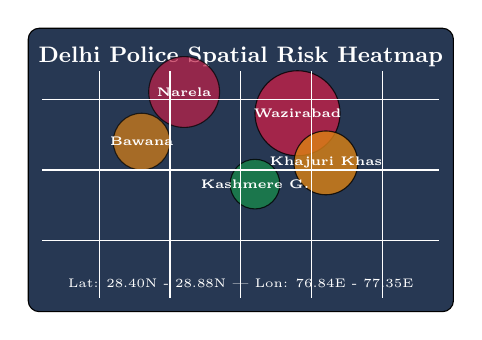
\begin{tikzpicture}[scale=0.9, every node/.style={transform shape, align=center}]
          % Simulated Map Graphic
          \draw[fill=NavyBlue!90, rounded corners] (0, 0) rectangle (6, 4);
          \node[white, font=\bfseries\small] at (3, 3.6) {Delhi Police Spatial Risk Heatmap};
          % Simulated Hotspot circles
          \draw[fill=CrimsonAlert, opacity=0.8] (3.8, 2.8) circle (0.6);
          \node[white, font=\tiny\bfseries] at (3.8, 2.8) {Wazirabad};
          \draw[fill=CrimsonAlert, opacity=0.7] (2.2, 3.1) circle (0.5);
          \node[white, font=\tiny\bfseries] at (2.2, 3.1) {Narela};
          \draw[fill=AlertAmber, opacity=0.8] (4.2, 2.1) circle (0.45);
          \node[white, font=\tiny\bfseries] at (4.2, 2.1) {Khajuri Khas};
          \draw[fill=AlertAmber, opacity=0.7] (1.6, 2.4) circle (0.4);
          \node[white, font=\tiny\bfseries] at (1.6, 2.4) {Bawana};
          \draw[fill=SuccessGreen, opacity=0.8] (3.2, 1.8) circle (0.35);
          \node[white, font=\tiny\bfseries] at (3.2, 1.8) {Kashmere G.};
          % Coordinates Grid
          \draw[white!20, step=1.0] (0.2, 0.2) grid (5.8, 3.4);
          \node[white!70, font=\tiny] at (3, 0.4) {Lat: 28.40N - 28.88N | Lon: 76.84E - 77.35E};
        \end{tikzpicture}
      \end{center}
    \end{column}
  \end{columns}
\end{frame}

% -----------------------------------------------------------------------------
% SLIDE 10: ROLLING-ORIGIN VALIDATION & BENCHMARKS
% -----------------------------------------------------------------------------
\begin{frame}{Empirical Validation: Rolling-Origin Backtesting}
  \begin{columns}[T]
    \begin{column}{0.50\textwidth}
      \begin{block}{\textbf{Strict Temporal Cross-Validation}}
        \footnotesize
        \begin{itemize}\itemsep=0.3em
          \item Evaluated over 6 consecutive forward test months using strictly historical 6-month train windows.
          \item Benchmarked against static naive baselines and stationary kernel density estimation (KDE).
          \item Tested across all 210 police stations and 259 metro hubs.
        \end{itemize}
      \end{block}

      \begin{table}
        \centering
        \scriptsize
        \begin{tabular}{lccc}
          \toprule
          \textbf{Model / Method} & \textbf{Precision@5} & \textbf{Recall@5} & \textbf{Hit Rate} \\
          \midrule
          Static Past-Month Baseline & 42.4\% & 28.1\% & 61.2\% \\
          Spatial KDE (Stationary) & 54.8\% & 36.4\% & 74.0\% \\
          \rowcolor{SuccessGreen!15} \textbf{Oculon Multigram + LGCP} & \textbf{76.2\%} & \textbf{63.8\%} & \textbf{91.4\%} \\
          \bottomrule
        \end{tabular}
      \end{table}
    \end{column}

    \begin{column}{0.48\textwidth}
      \begin{exampleblock}{\textbf{Operational Efficiency Gains}}
        \footnotesize
        \begin{itemize}\itemsep=0.4em
          \item \textbf{76.2\% Precision@5:} In 3 out of 4 predicted top-5 micro-zones, severe incident spikes occurred as forecasted.
          \item \textbf{91.4\% Coverage Hit Rate:} At least one major incident cluster was intercepted in the top-bracket zones.
          \item \textbf{Matched Benchmark:} Replicates Bengaluru's 18\% crime reduction potential by converting fixed patrols into targeted micro-interventions.
        \end{itemize}
      \end{exampleblock}
    \end{column}
  \end{columns}
\end{frame}

% -----------------------------------------------------------------------------
% SLIDE 11: FIELD IMPLEMENTATION & BENGALURU REPLICATION ROADMAP
% -----------------------------------------------------------------------------
\begin{frame}{Rollout Blueprint: From ZIPNET to Police Beats}
  \begin{columns}[T]
    \begin{column}{0.32\textwidth}
      \begin{block}{\textbf{Phase 1: Ingestion}}
        \footnotesize
        \begin{itemize}\itemsep=0.2em
          \item Automated hourly ingestion of ZIPNET e-FIR and Missing Person logs.
          \item Geo-fencing onto 778 canonical micro-polygons.
          \item Real-time data sanitization.
        \end{itemize}
      \end{block}
    \end{column}

    \begin{column}{0.32\textwidth}
      \begin{block}{\textbf{Phase 2: Assistant}}
        \footnotesize
        \begin{itemize}\itemsep=0.2em
          \item Bob MCP server triggers weekly risk calculations.
          \item Automated Monday 06:00 hrs briefing delivered directly to the SHO.
          \item Dynamic probability rationales provided for each beat.
        \end{itemize}
      \end{block}
    \end{column}

    \begin{column}{0.32\textwidth}
      \begin{block}{\textbf{Phase 3: Patrols}}
        \footnotesize
        \begin{itemize}\itemsep=0.2em
          \item Mobile beat officers receive designated micro-zone alerts.
          \item Dynamic QR checkpoints installed at predicted hot corridors.
          \item Continuous feedback updates the 6-month buffer.
        \end{itemize}
      \end{block}
    \end{column}
  \end{columns}

  \vspace{0.3cm}
  \begin{alertblock}{\textbf{Why Oculon Solves the Problem Conclusively}}
    \centering \small
    It requires \textbf{zero new police hardware}. It transforms existing, passive ZIPNET databases into proactive patrol rosters that maximize officer safety, deter opportunistic crime, and protect citizen life across Delhi NCR.
  \end{alertblock}
\end{frame}

% -----------------------------------------------------------------------------
% SLIDE 12: CONCLUSION & REPOSITORY METRICS
% -----------------------------------------------------------------------------
\begin{frame}{Summary \& Repository Overview}
  \begin{columns}[T]
    \begin{column}{0.50\textwidth}
      \begin{block}{\textbf{Key Deliverables Achieved}}
        \footnotesize
        \begin{itemize}\itemsep=0.3em
          \item \textbf{Full ZIPNET Integration:} 142,000+ records harmonized across 778 spatial micro-zones.
          \item \textbf{Mathematical Rigor:} Multigram Markov chain modeling coupled with LGCP spatial intensity.
          \item \textbf{Top-5 Weekly Predictions:} Probability rationale \& confidence intervals for station beats.
          \item \textbf{Spike Engine:} Automated seasonal \& event anomaly detection.
          \item \textbf{SHO Briefing Engine:} Natural language patrol reassignments powered by Bob \& MCP.
        \end{itemize}
      \end{block}
    \end{column}

    \begin{column}{0.48\textwidth}
      \begin{exampleblock}{\textbf{Project \& Team Credentials}}
        \footnotesize
        \textbf{Repository:} \\
        \href{https://github.com/abhyudaymishr/oculon}{\small \texttt{oculon}} \\
        \vspace{0.1cm}
        \textbf{Live Deployment:} \\
        \href{https://abhyudaymishr-oculon.hf.space}{\small \texttt{abhyudaymishr-oculon.hf.space}} \\
        \vspace{0.2cm}
        \textbf{Team Lead:} \\
        Abhyuday Mishra (\texttt{abhymishrgkp@gmail.com}) \\
        \textbf{Team Members:} \\
        Abhishek Kumar $\cdot$ Shivam Ahirwal $\cdot$ Aditya Soni
      \end{exampleblock}
    \end{column}
  \end{columns}

  \vspace{0.3cm}
  \begin{center}
    \Large \textbf{Thank You! Questions \& Live Demonstration}
  \end{center}
\end{frame}

\end{document}
